%\begin{myillus}

		Courbe représentative de la fonction $f(x) = \dfrac{1}{x}$ et tableau de variations associé:
	\begin{multicols}{2}

	


	\begin{center}
		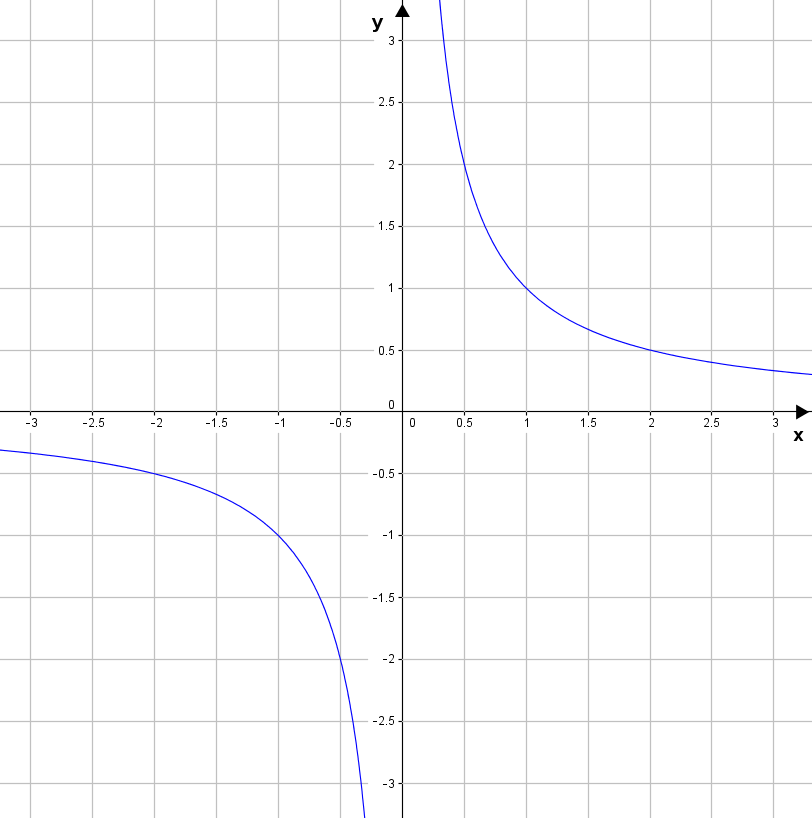
\includegraphics[scale=0.45]{./img/inverse}
	\end{center}
	
	

	\vspace*{0.5cm}
	\begin{center}
%		\begin{tikzpicture}
%		\tkzTabInit{$x$/1,$f(x)$/2}{$- \infty$,$0$,$+ \infty$}
%		%\tkzTabLine{,-,z,+}
%		\tkzTabVar{+/$+ \infty$,-/$0$,+/$+ \infty$}
%		\end{tikzpicture}	

		\begin{variations}
			x & \mI & & 0 & & \pI \\
			\filet
			\dfrac{1}{x} & \ga- & \bb & \dr+ \\				
		\end{variations}
		
		\vspace*{1cm}
		
		\begin{variations}
			x & \mI & & & 0 & & & \pI \\
		\filet
			\m{\dfrac{1}{x}} & \h\ & \d & \ & \bb & \h\ & \d & \ \\				
		\end{variations}
	\end{center}
	\end{multicols}
%\end{myillus}